\documentclass{article}

\usepackage[english]{babel}

% Set page size and margins
\usepackage[a4paper,top=2cm,bottom=2cm,left=3cm,right=3cm,marginparwidth=1.75cm]{geometry}

% Useful packages
\usepackage{amsmath}
\usepackage{graphicx}
\usepackage[colorlinks=true, allcolors=blue]{hyperref}


\title{Predicting the growth of crops using machine learning and time series analysis}

\begin{document}
\maketitle

\begin{table}[h]
    \centering
    \begin{tabular}{ll}
        Registration number: & \textcolor{red}{2105711}\\
        Project: & \textcolor{red}{(Agrotech)}\\
        Link to GitHub: & \url{https:}//github.com/pradeep5267/CE888/tree/main/agrotech
    \end{tabular}
\end{table}



\begin{table}[h]
    \centering
    \begin{tabular}{lc}
        Executive summary (max.\ 250 words) & \textcolor{red}{247}\\
        Introduction (max.\ 600 words) & \textcolor{red}{303}\\
        Data (max.\ 500 words/dataset) & \textcolor{red}{390}\\
        Methodology (max.\ 600 words) & \textcolor{red}{283}\\
        Conclusions (max.\ 500 words) & \textcolor{red}{83}\\
        \hline
        Total word count & \textcolor{red}{1306}\\
    \end{tabular}
    %\caption{Word counts for each section.}
\end{table}

\tableofcontents

\clearpage



\begin{abstract}
Given the objective to predict the plant size at a future date using historical data a good starting approach would be to identity what historical data features can be used. In this scenario the date at which the seed was planted, the weather in between the plant date and the date at which the drone measurements were taken would play an important role in determining the growth of the plant.\\As the objective requires to predict the size of the plants a regression model needs to be developed so that continuous values can be predicted by the trained model.\\The dateset provided contains 4 sheets from which the weather data has be chunked into smaller data-sets based on the year to develop weather predicting model. An ensemble of such models' average will be used as the output for weather prediction. After getting the weather features the missing features in the dataset will be imputed in using either an KNN model or a random forest regressor. Then an ensemble of models will be used to make the final predictions for the size of the plant. Care has been taken in dealing with weather data as to not include data from future ie 2020 onwards. The metrics used for evaluating the model will be R$^2$ and RMSE. However a dummy model will be developed to establish a baseline for determining the significance of the R$^2$ and RMSE scores. Hence ensemble regressor using multiple metrics would give the best outcome.
\end{abstract}


\section{Introduction}
As agriculture plays an important role in macro as well as micro economics, leveraging data science to make effective decisions not only shows the importance of data science in decision making but also enables the stake holder to be more flexible in taking the right decisions \cite{meinke2009adaptation}.
This project not only drives the above point forward but at the same time shows the importance of data driven decision making for the overall good. The objective, in simple terms is to predict whether the stake holder will be able to determine the quality and quantity of the produce at future date. The implications of making a wrong decision in such scenarios not only leads to a monetary loss to the stake holders but also results in food wastage which further implies a wastage of critical resources like water. Therefore the proposed model should be able to capture and approximate the trends found in the historical data to such a degree that given a new datapoint the model should be able to give an accurate output. This ensures that the right prediction is made for the given input date which reduces monetary loss and resource wastage. However the impact due to such data driven models is that not only the decision making process becomes highly efficient but also the entire supply chain operations.\\
Predicting the plant size at the right date not only ensure the stake holders don't face a monetary loss but it also ensures that monetary gains are made to due accurate reporting of the harvest, quantity and quality of produce to supermarkets. Thus using machine learning to make such decisions not only speeds up the decision making process and the accuracy of the decision made but also ensures that the intrinsic human bias doesnt play a big role in the decision making process \cite{mcqueen1995applying}.

\section{Data}
\begin{figure}[tb]
\centering
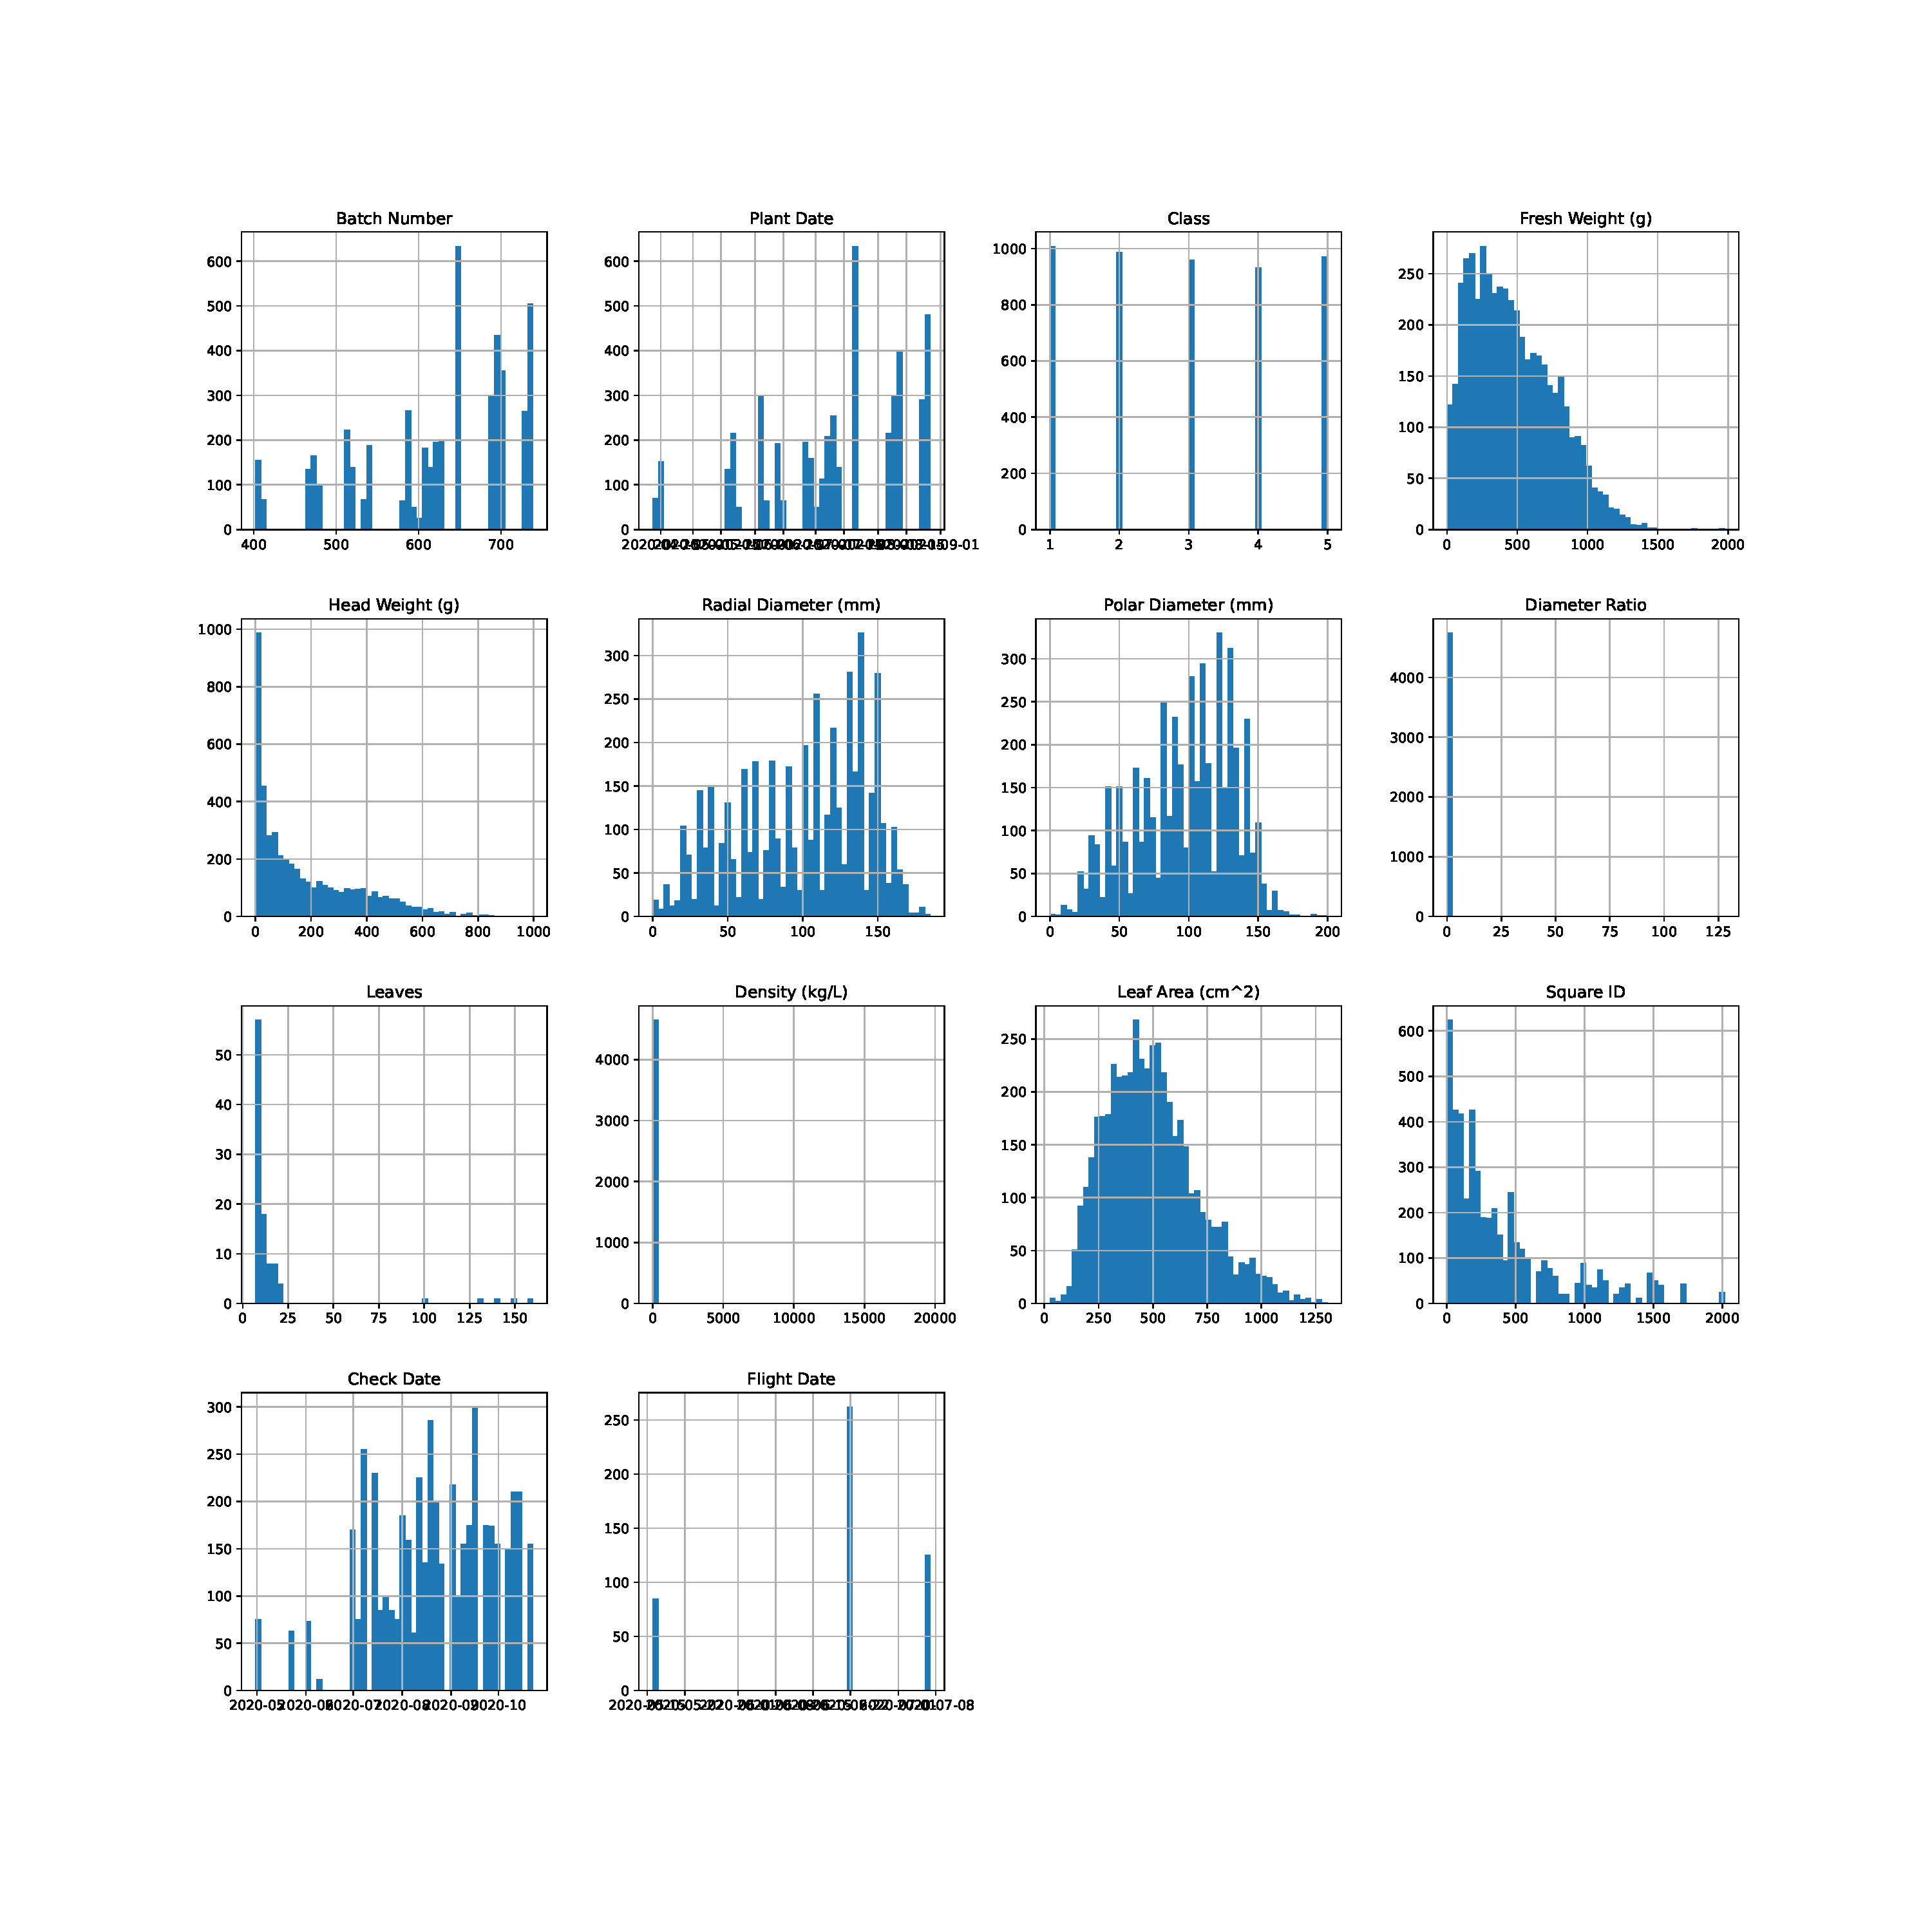
\includegraphics[width=0.7\textwidth]{plants_hist.pdf}
\caption{\label{fig:plants_hist}histogram plots of each column in plants dataframe.}
\end{figure}
The dataset used in this project is a private dataset provided by Dr. Ana Matran-Fernandez.\\
The dataset contains 4 sheets namely: plants, flight dates, planting, weather. Each of these sheets was loaded into a separate dataframe for easier exploration and manipulation of data.
As observed from above plots there are columns such as flight date. Since this is an important features and corresponding data is available from other dataframes, the required data is merged to get the required features in a single dataframe. In this case the data from flights dataframe is merged into plants dataframe using batch number as a key.\\
However for rows with plant date having empty value was dropped.\\
The plants dataset has 4859 datapoints having int, float and numpy datetime format columns.\\
New datetime feature was created for number of days from plant date to flight date. This will be useful as this period shows how long the crop took to grow to harvest-able quality. Some more date-time features were created like day, month and year features from plant date, flight date. These features will be used to calculate the mid date between plant and flight date which will be used to get weather features.\\
The weather dataset has 2556 entries having int, float and numpy datetime format columns. However some unimportant columns were also present like battery voltage which doesn't  directly quantify any weather feature and hence was dropped. Other columns like 'Wind Speed [max]', 'Air Temperature [max]', 'Air Temperature [min]', 'Dew Point [min]' were dropped as the min and max of such quantities vary a lot over a day. Therefore a better representation of such features would a summary statistic like mean and since mean of these features were present, the min and max features were dropped and mean was kept.\\
Coming back to the plants dataset, some important target features like head weight, polar and radial diameter were empty.
So two approaches can be tried here, one in which predicted weather features are used to along with other date and plant features to train a model which will then be used to impute values \cite{kuhn2019feature}. This dataset will then be used to train the ensemble regressor for final predictions. Second approach is to drop the rows where the above columns are empty and then train a regressor model without imputing the missing data.                                                                                                                                                                                                                                                                                                             
\section{Methodology}
\begin{figure}[tb]
\centering
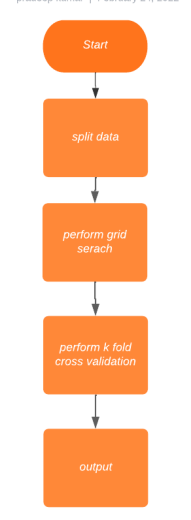
\includegraphics[scale=0.5]{flowchart.png}
\caption{\label{fig:flowchart}basic flow of training the model.}
\end{figure}
As the final outcome of this project is to predict the size of the crop a regression model has to be trained. A good model should be able to give satisfactory results on unseen data which implies that the model should not overfit while at the same time learn the underlying trends of the dataset.

\subsection{Baseline}
Since the metrics used for evalution will be R$^2$ and RMSE values, creating a baseline model would give a fair idea of how well the final trained model is performing when compared to baseline model.\\
The baseline model will be random forest regressor with no cross validation and no grid search performed.The dataset would be split into 70, 20 and 10 percent respectively for train, test and validation split. Then the random forest regressor will be trained on the training dataset.

\subsection{Model training}
The model training will also follow similar steps as that of the baseline model with the addition of grid search on parameters and k fold cross validation.\\
The ensemble model will be trained on the train dataset, however a grid search will be performed before training to determine the best parameters. After finding the best parameters the model will be trained using training set.\\
Same steps will be followed for creating other machine learning models too such as multi label linear regressors. All of the trained models will be evaluated to determine the best performing model.

\subsection{Evaluation of models}
The different trained models will then be evaluated using k fold cross validation (k = 10) to determine how well each model performs \cite{rodriguez2009sensitivity}. Evaluation metrics like RMSE and R$^2$ values will also be used.  Other techniques like bootstrapping can be used however its effective when the data set is small in size.

\section{Conclusions}
As the dataset reflects a real world issue, developing a data driven solution has the potential to lead to a real world impact. A model with low enough RMSE should be able to give pretty good outputs. However further experimentation with weather features and imputation of radial, polar diameter needs to be carried out to determine the best features for training the model. Neural networks have also shown very promising results \cite{bhojani2020wheat} so throwing these into the mix should lead to quite useful outcome.





\bibliographystyle{abbrv}
\bibliography{name.bib}

\end{document}